\section{CHƯƠNG 6: DASHBOARD PHÂN TÍCH USER}


Dashboard này nhằm khám phá và phân tích dữ liệu về các nhà sáng tạo nội dung trên TikTok. Phần này cung cấp cái nhìn tổng quan về bộ dữ liệu thu thập được.

\begin{itemize}
    \item Tổng số TikToker: 264 người
    \item Số người theo dõi trung bình: 336,473
    \item Số lượt thích trung bình: 10,214,598
    \item Số lượng video trung bình: 550 video
\end{itemize}

Dựa trên các con số này, nếu thu thập toàn bộ video của các TikToker, bộ dữ liệu sẽ bao gồm khoảng $264 \times 550 = 145{,}200$ video. Đây là một khối lượng dữ liệu đáng kể, đủ để xác định xu hướng ngành, đề xuất chiến lược nội dung, cũng như so sánh hiệu suất giữa các nhóm TikToker. Tuy nhiên, do hạn chế về thời gian và năng lực xử lý, phân tích trong báo cáo này sẽ tập trung vào các video mới và có nội dung liên quan trực tiếp đến chủ đề ẩm thực.


\textbf{Nhận xét:} Số lượt thích trung bình và số người theo dõi khá cao, đặt ra câu hỏi liệu dữ liệu có bị mất cân bằng hay không. Nếu có, cần áp dụng các phương pháp phân tích cẩn thận để đảm bảo kết quả thuyết phục.

\subsection{Phân phối của dữ liệu}


\subsubsection{Phân Phối Số Lượt Thích}
\begin{figure}[H]
    \centering
    \fcolorbox{gray}{white}{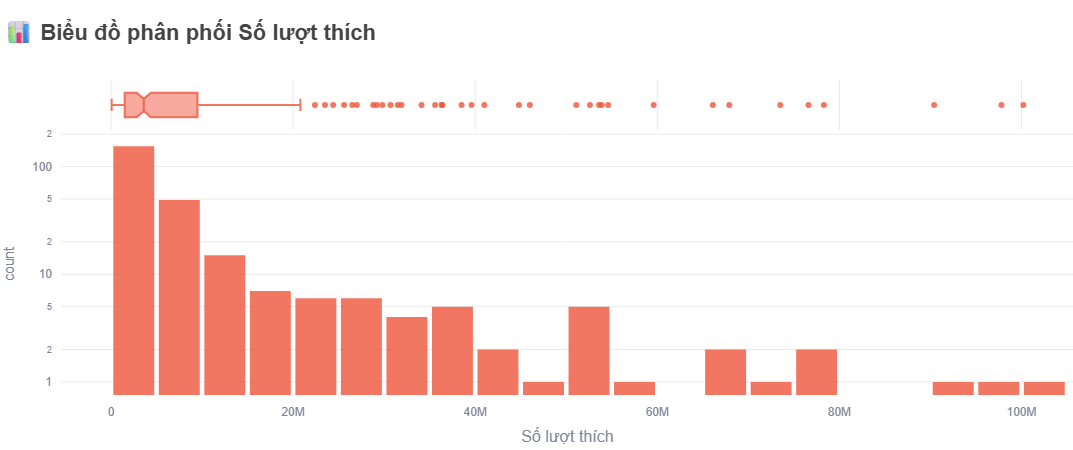
\includegraphics[width=0.8\textwidth]{img/phan_phoi_so_luot_thich.png}}
    \caption{Phân Phối Số Lượt Thích}
    \label{fig:phan_phoi_luot_thich}
\end{figure}

\noindent
Phân phối số lượt thích (Hình~\ref{fig:phan_phoi_luot_thich}) có dạng lệch phải, với các đặc điểm:
\begin{itemize}
    \item Hầu hết video có số lượt thích thấp, nhưng giá trị trung bình (hơn 10 triệu) bị kéo lên bởi một số video có lượt thích cực cao.
    
    \item Khoảng tứ phân vị (IQR): từ 1.5 triệu (Q1) đến 9.5 triệu (Q3), cho thấy sự phân tán lớn.
    
    \item Giá trị tối đa: 100.2 triệu, nhấn mạnh sự hiện diện của các giá trị ngoại lai ảnh hưởng mạnh đến trung bình.
\end{itemize}

\subsubsection{Phân Phối Số Người Theo Dõi}
\begin{figure}[H]
    \centering{
    \fcolorbox{gray}{white}{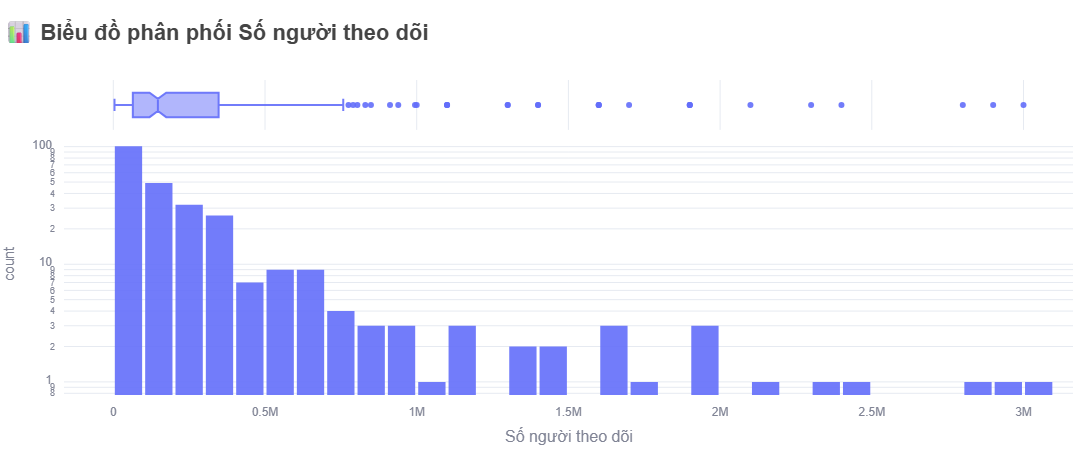
\includegraphics[width=0.8\textwidth]{img/phan_phoi_so_luot_theo_doi.png}}
    \caption{Phân phối số người theo dõi}
    \label{fig:phan_phoi_luot_theo_doi}
    }
\end{figure}

\noindent
Phân phối số người theo dõi (Hình~\ref{fig:phan_phoi_luot_theo_doi}) có tính bất đối xứng cao và lệch phải:
\begin{itemize}
    \item Phần lớn tài khoản có số người theo dõi thấp, với đuôi phải kéo dài đến các giá trị lớn.
    
    \item Trung bình: $\sim$336,000, cao hơn nhiều so với trung vị ($\sim$147,000), do ảnh hưởng của một số tài khoản rất nổi tiếng.
    
    \item Giá trị tối đa: 3 triệu, cho thấy sự chênh lệch lớn về mức độ nổi tiếng giữa các TikToker.
\end{itemize}

\textbf{Nhận xét:} Phân phối này tương tự phân phối mũ hoặc lũy thừa, nơi số người theo dõi tăng theo cấp số nhân ở một số ít tài khoản.

\subsubsection{Phân Phối Số Lượng Video}

\noindent
Phân phối số lượng video (Hình~\ref{fig:phan_phoi_so_luong_video}) có dạng lệch phải, với các đặc điểm:
\begin{itemize}
    \item Trung vị: 460 video.
    
    \item Khoảng tứ phân vị (IQR): từ 256 đến 752 video.
    
    \item Trung bình: 549.64, cao hơn trung vị, do một số TikToker có số lượng video rất lớn.
    
    \item Độ lệch chuẩn: 409.13, thể hiện sự khác biệt đáng kể về số lượng video.
    
    \item Giá trị tối đa: 2,298 video, cho thấy có những người dùng rất tích cực.
\end{itemize}

\begin{figure}[ht]
    \centering
    \fcolorbox{gray}{white}{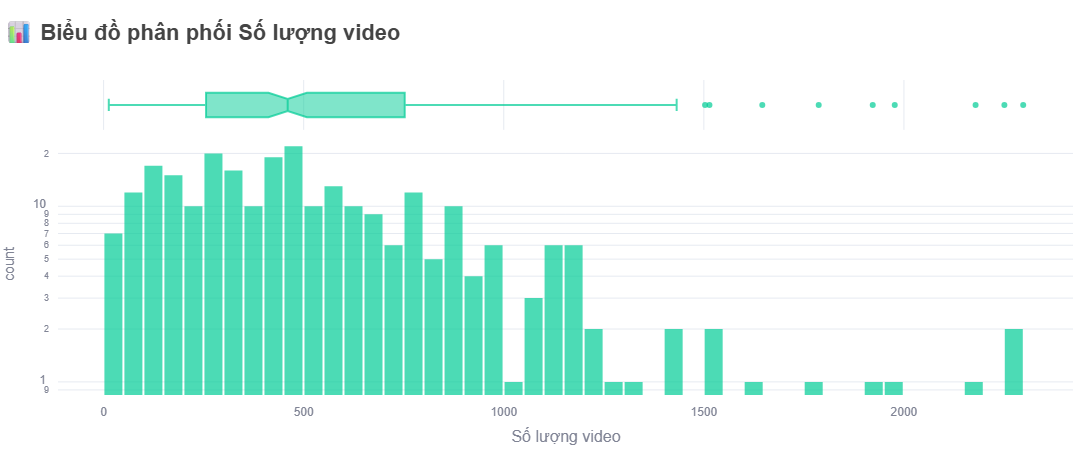
\includegraphics[width=0.8\textwidth]{img/phan_phoi_so_luong_video.png}}
    \caption{Phân phối số lượng video}
    \label{fig:phan_phoi_so_luong_video}
\end{figure}

\vspace*{-10pt}
\subsection{Phân Tích Tương Quan}

\noindent
Cùng quan sát hai biểu đồ sau:

\vspace*{-4pt}
\begin{figure}[ht]
    \centering
    \fcolorbox{gray}{white}{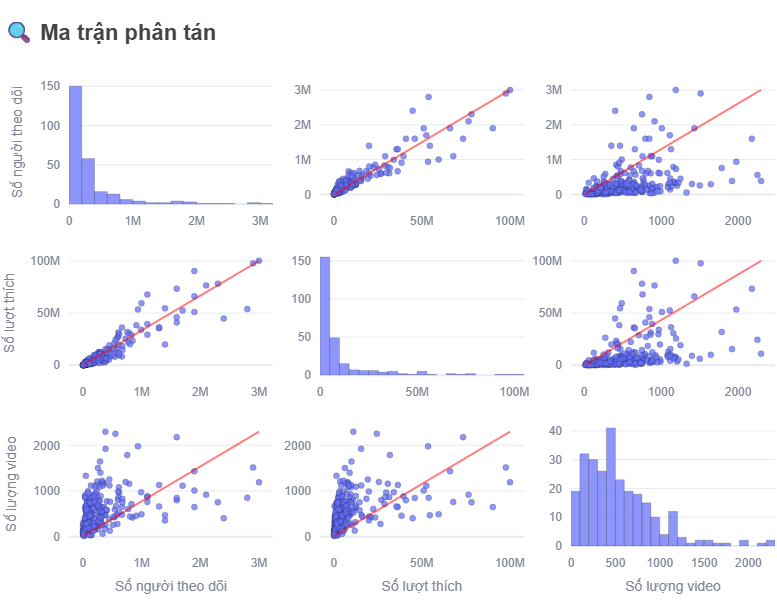
\includegraphics[width=0.80\textwidth]{img/ma_tran_phan_tan.png}}
    \caption{Ma Trận Phân Tán}
    \label{fig:ma_tran_phan_tan}
\end{figure}

\begin{figure}[H]
    \centering
    \fcolorbox{gray}{white}{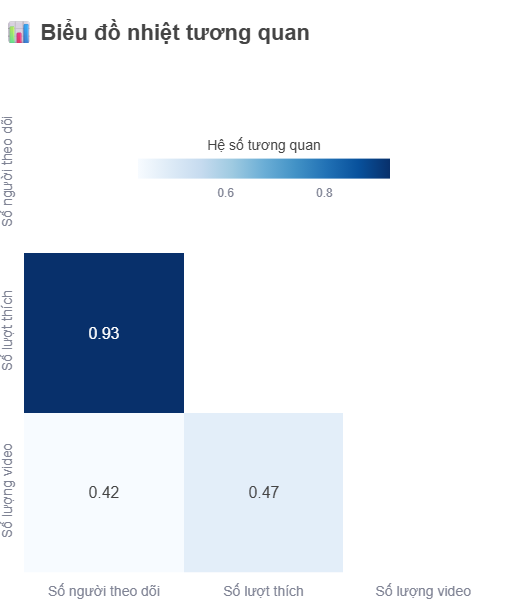
\includegraphics[width=0.6\textwidth]{img/bieu_do_nhiet_tuong_quan.png}}
    \caption{Biểu Đồ Nhiệt Tương Quan}
    \label{fig:bieu_do_nhiet_tuong_quan}
\end{figure}

Mức độ tương quan giữa các cặp biến khác nhau đáng kể. Có thể thấy một tương quan mạnh mẽ giữa `Số người theo dõi' và `Số lượt thích', cùng với tương quan vừa phải giữa `Số người theo dõi' và `Số lượng video', cũng như `Số lượt thích' và `Số lượng video'.

\begin{itemize}
    \item \textbf{`Số người theo dõi' và `Số lượt thích':} Mối tương quan giữa `Số người theo dõi' và `Số lượt thích' là rất mạnh (0.933). Điều này cho thấy mối quan hệ dương tính: khi một TikToker có nhiều người theo dõi, các video của họ cũng thường nhận được nhiều lượt thích hơn. Điều này có thể là do những người theo dõi thường xuyên xem và tương tác với nội dung của tài khoản, hoặc do các thuật toán ưu tiên hiển thị nội dung của các tài khoản có lượng theo dõi lớn, dẫn đến tăng lượt thích.
    
    \item \textbf{`Số người theo dõi' và `Số lượng video':} Mối tương quan giữa `Số người theo dõi' và `Số lượng video' là trung bình (0.422). Tương quan dương cho thấy, nhìn chung, những TikToker đăng nhiều video hơn có xu hướng có lượng người theo dõi lớn hơn. Điều này có thể là do việc đăng tải thường xuyên giúp tăng khả năng hiển thị trên nền tảng và thu hút thêm người xem. Tuy nhiên, mối tương quan này không quá mạnh, có thể có những TikToker với số lượng video hạn chế nhưng vẫn thu hút được lượng lớn người theo dõi nhờ chất lượng nội dung.
    
    \item \textbf{`Số lượt thích' và `Số lượng video':} Mối tương quan giữa `Số lượt thích' và `Số lượng video' cũng là trung bình (0.473). Mối tương quan dương này ám chỉ những TikToker đăng nhiều video có xu hướng nhận được nhiều lượt thích hơn. Điều này có thể phản ánh sự hiện diện thường xuyên hơn trên nền tảng dẫn đến việc video có cơ hội hiển thị nhiều hơn và được nhiều lượt thích hơn.
\end{itemize}

\paragraph{Kết Luận và Gợi Ý:}
Người sáng tạo nội dung TikTok nên tập trung vào việc xây dựng lượng người theo dõi chất lượng, bởi vì nó có liên quan mật thiết với tương tác (lượt thích) trên các video. Đồng thời, việc đăng tải video thường xuyên, kết hợp với việc nâng cao chất lượng nội dung, có thể là một chiến lược hiệu quả để gia tăng cả lượng người theo dõi và lượt tương tác. Để đạt được kết quả tốt nhất, nhà sáng tạo nên tập trung vào việc tạo ra những video chất lượng cao, được đầu tư kỹ lưỡng về nội dung, hình ảnh và âm thanh để thu hút người xem.

\subsection{Phân Tích Mức Độ Tương Tác Theo Nhóm Người Theo Dõi}
Như vậy, qua phân tích tổng quát, chúng ta có thể thấy dữ liệu được thu thập có phân phối bất đối xứng và xu hướng lệch phải. Do đó để các phân tích có tính thuyết phục, chúng ta sẽ tiến hành phân chia các TikToker theo nhóm dựa trên lượng người theo dõi, để có thể khám phá ra các đặc điểm, tính chất để các kết luận đưa ra được tăng tính thuyết phục.

\subsubsection{Phân Chia Nhóm Người Theo Dõi}
\begin{itemize}
    \item \textbf{Nhóm người theo dõi thấp:} Những người dùng có số người theo dõi thấp hơn 85,627. Những người dùng này có thể là những người mới bắt đầu hoặc chưa có nhiều nội dung nổi bật.
    
    \item \textbf{Nhóm người theo dõi trung bình:} Những người dùng có số người theo dõi nằm trong khoảng 85,627 - 276,358. Những người dùng này có thể là những người mới nổi hoặc có ảnh hưởng vừa phải trên TikTok.
    
    \item \textbf{Nhóm người theo dõi cao:} Những người dùng có số người theo dõi cao hơn 276,358. Những người dùng này có thể là những người nổi tiếng hoặc có ảnh hưởng lớn trên TikTok.
\end{itemize}

\subsubsection{Bảng So Sánh Mức Độ Tương Tác}
\begin{table}[H]
    \centering
    \begin{tabular}{lccc}
        \toprule
        Chỉ số & Thấp & Trung bình & Cao \\
        \midrule
        Số mẫu & 87 & 87 & 90 \\
        Số người theo dõi & 45,665 & 160,687 & 787,512 \\
        Số lượt xem trên mỗi video & 195,285 & 371,054 & 729,571 \\
        Số bình luận trên mỗi video & 99 & 176 & 238 \\
        Số lượt thích trên mỗi video & 5,362 & 11,633 & 35,050 \\
        Số lượt chia sẻ trên mỗi video & 556 & 1,039 & 960 \\
        Số lượt lưu trên mỗi video & 766 & 1,293 & 1,772 \\
        Số video mỗi tuần & $4.4 \pm 4.0$ & $4.5 \pm 2.4$ & $4.7 \pm 2.4$ \\
        Số hashtag trên mỗi video & $7.5 \pm 2.5$ & $6.8 \pm 2.5$ & $5.7 \pm 2.1$ \\
        Thời lượng video (giây) & $59.0 \pm 36.3$ & $74.5 \pm 47.1$ & $103.6 \pm 59.6$ \\
        \bottomrule
    \end{tabular}
    \caption{So sánh mức độ tương tác của TikToker theo số người theo dõi}
    \label{tab:so_sanh_tuong_tac}
\end{table}

\paragraph{Nhận xét:}
\begin{itemize}
    \item \textbf{Tương tác tăng theo số người theo dõi:} TikToker có số người theo dõi cao (787,512) đạt mức tương tác vượt trội ở hầu hết các chỉ số (lượt xem, bình luận, lượt thích, lưu) so với nhóm trung bình (160,687) và thấp (45,665). Riêng số lượt chia sẻ của nhóm cao (960) thấp hơn nhóm trung bình (1,039), có thể do đặc điểm nội dung hoặc đối tượng khán giả.
    
    \item \textbf{Tần suất đăng video:} Số video mỗi tuần tăng nhẹ từ nhóm thấp (4.4) đến nhóm cao (4.7), với độ biến thiên giảm (từ $\pm$4.0 xuống $\pm$2.4), cho thấy nhóm có nhiều người theo dõi hơn có xu hướng duy trì lịch đăng ổn định hơn.
    
    \item \textbf{Số hashtag:} Nhóm thấp sử dụng nhiều hashtag hơn (7.5) so với nhóm trung bình (6.8) và cao (5.7), có thể do nỗ lực tăng khả năng hiển thị. Nhóm cao ít sử dụng hashtag hơn, có thể do đã có lượng khán giả sẵn có và ít phụ thuộc vào khám phá qua hashtag.
    
    \item \textbf{Thời lượng video:} Thời lượng video tăng rõ rệt từ nhóm thấp (59.0 giây) đến nhóm cao (103.6 giây), với độ biến thiên cũng tăng (từ $\pm$36.3 đến $\pm$59.6). Điều này cho thấy nhóm có nhiều người theo dõi hơn thường sản xuất video dài hơn và đa dạng hơn về độ dài.
\end{itemize}


\subsection{Ảnh Hưởng của Số Lượng Video Đến Tương Tác}
\textbf{Câu hỏi:} Với cùng một ngưỡng số người theo dõi nhất định, liệu việc tăng số lượng video có thực sự đem lại nhiều lượt xem và lượt tương tác hơn trên mỗi video, hay chỉ đơn thuần tạo ra nhiều lượt xem và tương tác tổng?

\begin{figure}[H]
    \centering
    \fcolorbox{gray}{white}{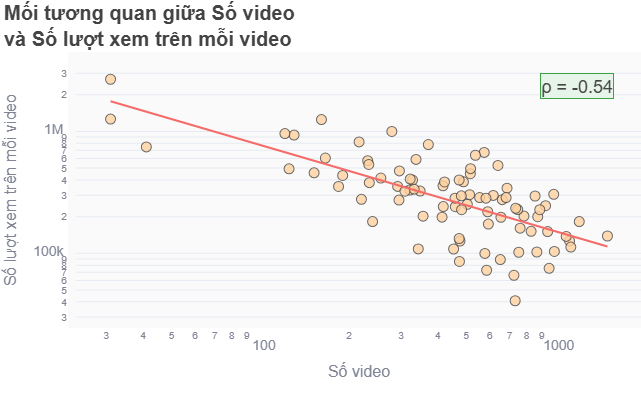
\includegraphics[width=0.82\textwidth]{img/so_video_so_luot_xem_nhom_TB.png}}
    \caption{Mối tương quan giữa số Video và số Luợt xem ở nhóm Tiktoker có lượng người theo dõi trung bình}
    \label{fig:so_video_luot_xem_nhom_TB}
\end{figure}

\begin{figure}[H]
    \centering
    \fcolorbox{gray}{white}{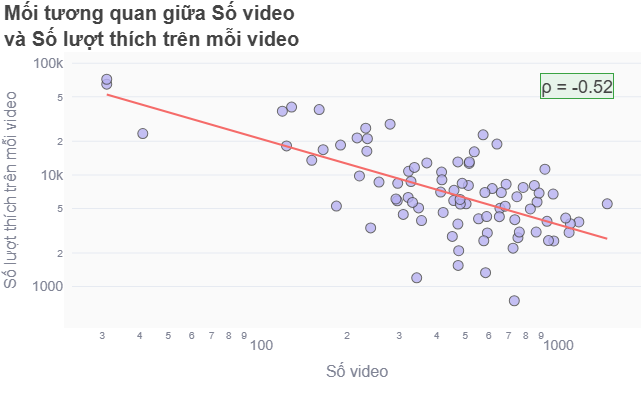
\includegraphics[width=0.82\textwidth]{img/so_video_so_luot_thich_nhom_TB.png}}
    \caption{Mối tương quan giữa số Video và số Luợt thích ở nhóm Tiktoker có lượng người theo dõi trung bình}
    \label{fig:so_video_luot_thich_nhom_TB}
\end{figure} 

\begin{figure}[H]
    \centering
    \fcolorbox{gray}{white}{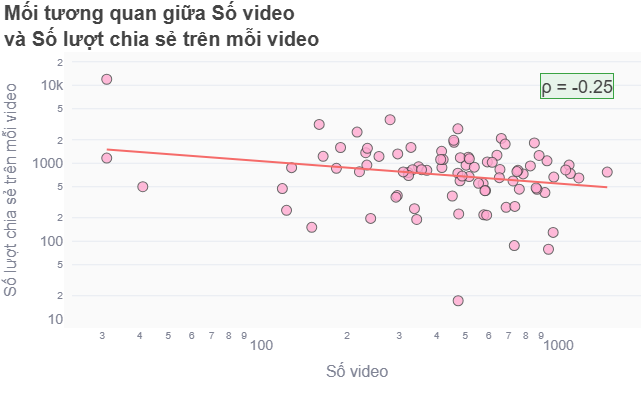
\includegraphics[width=0.82\textwidth]{img/so_video_so_luot_chia_se__nhom_TB.png}}
    \caption{Mối tương quan giữa số Video và số Luợt chia sẻ ở nhóm Tiktoker có lượng người theo dõi trung bình}
    \label{fig:so_video_luot_chia_se_nhom_TB}
\end{figure}

\begin{figure}[H]
    \centering
    \fcolorbox{gray}{white}{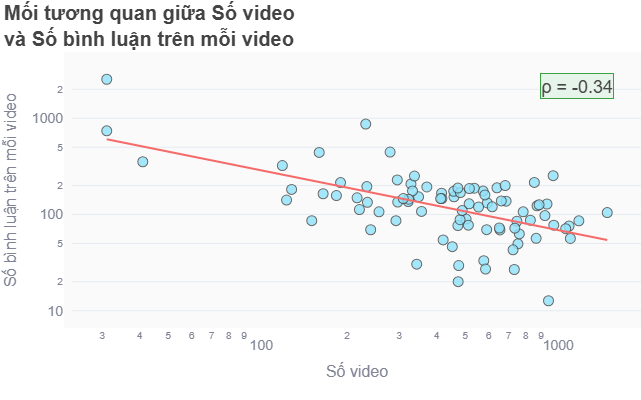
\includegraphics[width=0.82\textwidth]{img/so_video_so_binh_luan_nhom_TB.png}}
    \caption{Mối tương quan giữa số Video và số Luợt bình luận ở nhóm Tiktoker có lượng người theo dõi trung bình}
    \label{fig:so_video_binh_luan_nhom_TB}
\end{figure}


Qua phân tích mối tương quan giữa Tổng số video đăng tải và các chỉ số Lượt xem/Lượt thích/Lượt bình luận/Lượt chia sẻ trung bình trên mỗi video, một xu hướng nhất quán đã được quan sát và có thể tổng quát hóa cho cả ba nhóm người dùng (Thấp, Trung bình, Cao về số người theo dõi):

\subsubsection*{Mối tương quan nghịch giữa Số lượng video và Tương tác trên mỗi video:}

Đối với tất cả các chỉ số tương tác được phân tích (Lượt xem, Lượt thích, Lượt bình luận, Lượt chia sẻ), đều tồn tại mối tương quan nghịch với tổng số lượng video đăng tải. Điều này có nghĩa là, nhìn chung, khi một TikToker đăng tải càng nhiều video, thì lượng tương tác trung bình (lượt xem, lượt thích, bình luận, chia sẻ) mà mỗi video riêng lẻ nhận được có xu hướng giảm xuống.

Mối tương quan nghịch này thể hiện rõ nhất ở Lượt xem và Lượt thích, và yếu dần ở Lượt bình luận và Lượt chia sẻ. Điều này cho thấy việc tăng số lượng video tác động mạnh hơn đến lượt xem và lượt thích trên từng video so với lượt bình luận và chia sẻ.

Đường xu hướng trên các biểu đồ phân tán đều minh họa xu hướng giảm của tương tác trên mỗi video khi số lượng video tăng lên.

\subsubsection*{Sự đánh đổi giữa Số lượng và Chất lượng (trên mỗi video):}

Kết quả này nhấn mạnh sự đánh đổi tiềm ẩn giữa số lượng và hiệu quả tương tác trên từng video. Mặc dù việc đăng nhiều video hơn có thể làm tăng tổng số lượt xem/tương tác kênh nhận được (do số lượng nội dung nhiều hơn), nó dường như lại làm "loãng" mức độ tương tác trung bình mà mỗi video đơn lẻ có thể thu hút.

Quan sát về các TikToker có ít video nhưng đạt lượt tương tác trung bình trên mỗi video rất cao (nằm ở góc trên bên trái của các biểu đồ phân tán) củng cố nhận định này. Những nhà sáng tạo này có thể đang tập trung vào việc sản xuất nội dung chất lượng cao, độc đáo, hoặc tìm được thị trường ngách hiệu quả, giúp tối đa hóa hiệu quả tương tác của từng video mà không cần đăng bài ồ ạt.

\paragraph{Hàm ý cho Nhà sáng tạo nội dung (Tổng quát cho mọi nhóm):}
Dựa trên mối tương quan nghịch được quan sát, chiến lược "chất lượng hơn số lượng" (trên mỗi video) dường như là một yếu tố quan trọng để tối đa hóa mức độ tương tác trung bình cho từng nội dung.
\begin{itemize}
    \item \textbf{Ưu tiên Chất lượng Nội dung:} Thay vì chỉ tập trung vào việc tăng tần suất đăng bài để có nhiều nội dung hơn, các nhà sáng tạo ở mọi nhóm (Thấp, Trung bình, Cao) nên ưu tiên đầu tư thời gian, công sức vào việc sản xuất các video có chất lượng cao, hấp dẫn, độc đáo và phù hợp với đối tượng mục tiêu.
    
    \item \textbf{Tối ưu hóa Tương tác trên từng Video:} Chú trọng vào các yếu tố giúp tăng tương tác trên mỗi video như nội dung giá trị, hình ảnh/âm thanh thu hút, kêu gọi hành động (call-to-action) rõ ràng, tương tác với bình luận của người xem, v.v..
    
    \item \textbf{Cân bằng giữa Số lượng và Chất lượng:} Nhà sáng tạo cần tìm ra sự cân bằng phù hợp giữa tần suất đăng bài đều đặn và việc duy trì chất lượng cho từng video để tối ưu hóa cả tổng tương tác kênh và hiệu quả của từng nội dung.
\end{itemize}

\paragraph{Kết luận:}
Phân tích này cho thấy một xu hướng rõ ràng: việc tăng tổng số lượng video đăng tải có mối liên hệ tiêu cực với hiệu quả tương tác trung bình trên mỗi video. Điều này nhấn mạnh tầm quan trọng của chất lượng nội dung và chiến lược tối ưu hóa từng video đối với các nhà sáng tạo TikTok, bất kể họ đang ở mức độ người theo dõi nào.


\subsection{Phân tích ý nghĩa thống kê về tần suất đăng tải video mỗi tuần, số lượng hashtag trung bình trên mỗi video và thời lượng video trung bình giữa các nhóm người dùng}

\textbf{Câu hỏi nghiên cứu:}
Có sự khác biệt có ý nghĩa thống kê về tần suất đăng tải video mỗi tuần, số lượng hashtag trung bình trên mỗi video và thời lượng video trung bình giữa các nhóm người dùng có số người theo dõi thấp, trung bình và cao không?

\subsubsection{Về Tần Suất Đăng Tải Video Mỗi Tuần}

\begin{figure}[H]
    \centering
    \fcolorbox{gray}{white}{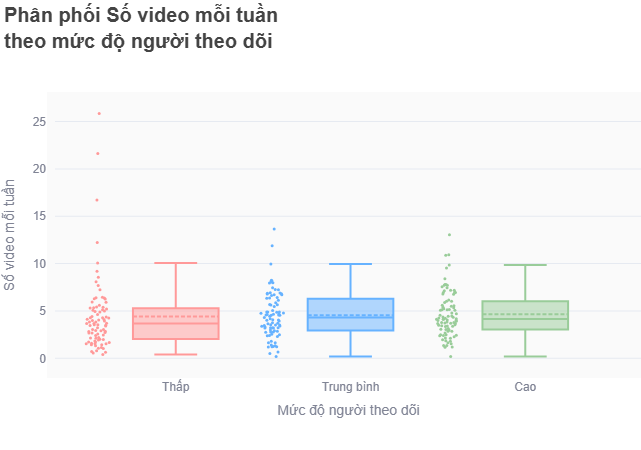
\includegraphics[width=0.7\textwidth]{img/so_video_moi_tuan_theo_nguoi_theo_doi.png}}
    \caption{Phân phối Số Video Mỗi Tuần theo Mức Độ Người Theo Dõi}
    \label{fig:so_video_tuan_phan_phoi}
\end{figure}

\begin{figure}[H]
    \centering
    \fcolorbox{gray}{white}{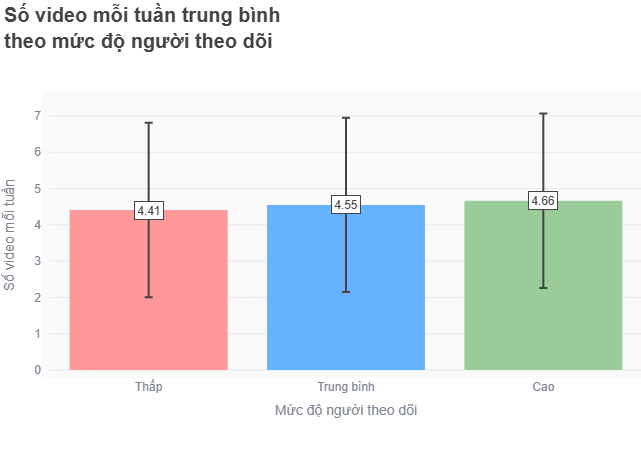
\includegraphics[width=0.7\textwidth]{img/so_video_trung_binh_moi_tuan_theo_nguoi_theo_doi.png}}
    \caption{Số Video Trung Bình Mỗi Tuần theo Mức Độ Người Theo Dõi}
    \label{fig:so_video_tuan_trung_binh}
\end{figure}

\begin{table}[H]
    \centering
    \begin{tabular}{lccccc}
        \toprule
        Mức độ người theo dõi & Số lượng mẫu & Trung bình & Độ lệch chuẩn & Tối thiểu & Tối đa \\
        \midrule
        Thấp & 87 & 4.41 & 4.00 & 0.42 & 25.85 \\
        Trung bình & 87 & 4.55 & 2.44 & 0.20 & 13.65 \\
        Cao & 90 & 4.66 & 2.40 & 0.19 & 13.05 \\
        \bottomrule
    \end{tabular}
    \caption{Thống kê Mô tả Số Video Mỗi Tuần theo Mức Độ Người Theo Dõi}
    \label{tab:so_video_tuan_thong_ke}
\end{table}

\paragraph{Kết quả kiểm định thống kê:}
Kiểm định Kruskal-Wallis: $p$-value = 0.0856
\begin{itemize}
    \item \textbf{Kết luận:} Không có sự khác biệt có ý nghĩa thống kê về Số video mỗi tuần giữa các nhóm người dùng có số lượng người theo dõi khác nhau ($p = 0.0856 > 0.05$).
\end{itemize}

\paragraph{Nhận xét:} Dựa trên kết quả kiểm định và các thống kê mô tả:
\begin{itemize}
    \item \textbf{Không có sự khác biệt ý nghĩa:} Giá trị $p$-value = 0.0856 lớn hơn mức ý nghĩa thông thường (ví dụ: 0.05). Điều này cho thấy không có bằng chứng thống kê thuyết phục để kết luận rằng có sự khác biệt đáng kể về số video mỗi tuần giữa các nhóm người dùng có số lượng người theo dõi khác nhau (Thấp, Trung bình, Cao).
    
    \item \textbf{Xu hướng không rõ ràng:} Mặc dù không có ý nghĩa thống kê, các giá trị trung bình cho thấy một xu hướng tăng nhẹ về số video mỗi tuần khi số lượng người theo dõi tăng lên (4.41 $\rightarrow$ 4.55 $\rightarrow$ 4.66). Tuy nhiên, sự khác biệt này quá nhỏ và không đủ để kết luận chắc chắn.
    
    \item \textbf{Ý nghĩa đối với nhà sáng tạo nội dung:} Kết quả này gợi ý rằng số lượng người theo dõi hiện tại có thể không phải là yếu tố quyết định chính trong việc xác định tần suất đăng video của một người dùng. Điều này có thể vì các nhà sáng tạo nội dung ở tất cả các quy mô theo dõi đều đăng video ở tần suất tương tự.
\end{itemize}

\paragraph{Chiến lược gợi ý:}
\begin{itemize}
    \item \textbf{Tập trung vào chất lượng:} Thay vì chỉ tập trung vào việc tăng tần suất đăng video, các nhà sáng tạo nên tập trung vào việc tạo ra nội dung chất lượng, thu hút và phù hợp với đối tượng khán giả mục tiêu.
    
    \item \textbf{Kiểm tra và thử nghiệm:} Cần tiếp tục theo dõi và phân tích dữ liệu để hiểu rõ hơn về hành vi của khán giả và tìm ra tần suất đăng video tối ưu. Có thể thử nghiệm các chiến lược khác, như đăng video vào các thời điểm khác nhau trong tuần hoặc thử nghiệm các loại nội dung khác nhau để xem xét ảnh hưởng.
    
    \item \textbf{Các yếu tố khác:} Ngoài số lượng người theo dõi, các yếu tố khác như tương tác (like, comment, share), nội dung, thời điểm đăng tải và thuật toán của TikTok có thể đóng vai trò quan trọng hơn trong việc quyết định sự thành công của một video.
\end{itemize}

\subsubsection{Về Số Lượng Hashtag}

\begin{figure}[H]
    \centering
    \fcolorbox{gray}{white}{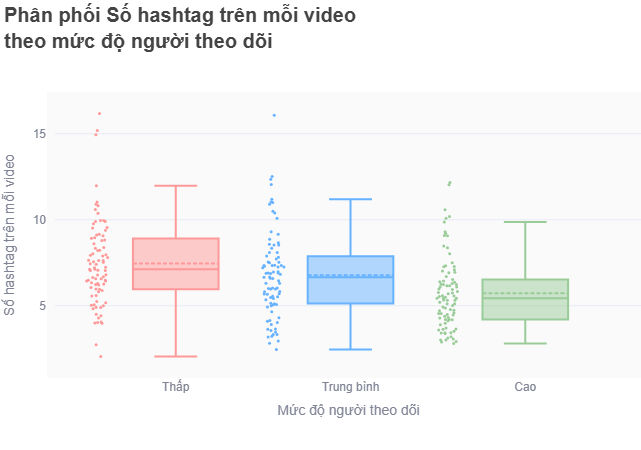
\includegraphics[width=0.7\textwidth]{img/so_hastag_tren_moi_video_theo_muc_do_nguoi_theo_doi.png}}
    \caption{Phân phối Số Hashtag trên Mỗi Video theo Mức Độ Người Theo Dõi}
    \label{fig:so_hashtag_phan_phoi}
\end{figure}

\begin{figure}[H]
    \centering
    \fcolorbox{gray}{white}{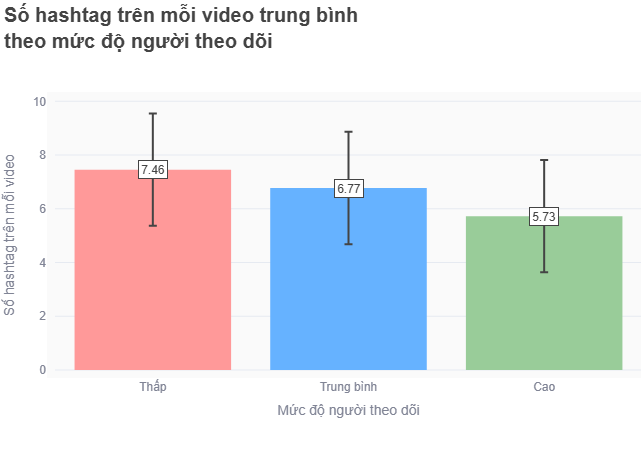
\includegraphics[width=0.7\textwidth]{img/so_hastag_trung_binh_tren_moi_video_theo_muc_do_nguoi_theo_doi.png}}
    \caption{Số Hashtag Trung Bình trên Mỗi Video theo Mức Độ Người Theo Dõi}
    \label{fig:so_hashtag_trung_binh}
\end{figure}

\begin{table}[h!]
    \centering
    \begin{tabular}{lccccc}
        \toprule
        Mức độ người theo dõi & Số lượng mẫu & Trung bình & Độ lệch chuẩn & Tối thiểu & Tối đa \\
        \midrule
        Thấp & 87 & 7.46 & 2.50 & 2.04 & 16.18 \\
        Trung bình & 87 & 6.77 & 2.52 & 2.46 & 16.07 \\
        Cao & 90 & 5.73 & 2.09 & 2.80 & 12.16 \\
        \bottomrule
    \end{tabular}
    \caption{Thống kê Mô tả Số Hashtag trên Mỗi Video theo Mức Độ Người Theo Dõi}
    \label{tab:so_hashtag_thong_ke}
\end{table}

\paragraph{Kết quả kiểm định thống kê:}
Kiểm định Kruskal-Wallis: $p$-value = 0.0000
\begin{itemize}
    \item \textbf{Kết luận:} Có sự khác biệt có ý nghĩa thống kê về Số hashtag trên mỗi video giữa các nhóm người dùng có số lượng người theo dõi khác nhau ($p = 0.0000 < 0.05$).
\end{itemize}

\paragraph{Nhận xét:}
\begin{itemize}
    \item \textbf{Sự khác biệt có ý nghĩa thống kê:} $p$-value = 0.0000 cho thấy có sự khác biệt có ý nghĩa thống kê giữa các nhóm người dùng về số lượng hashtag trên mỗi video. Điều này cho thấy mối quan hệ giữa số lượng người theo dõi và việc sử dụng hashtag không phải là ngẫu nhiên.

    \item \textbf{Số hashtag cao nhất/thấp nhất:}
    \begin{itemize}
        \item Nhóm người theo dõi \textbf{Thấp}: Trung bình số hashtag là 7.46, cao nhất trong ba nhóm.
        \item Nhóm người theo dõi \textbf{Cao}: Trung bình số hashtag là 5.73, thấp nhất trong ba nhóm.
    \end{itemize}

    \item \textbf{Ý nghĩa đối với nhà sáng tạo nội dung:} Những nhà sáng tạo có ít người theo dõi có xu hướng sử dụng nhiều hashtag hơn. Điều này có thể là một nỗ lực để tăng khả năng hiển thị video của họ trong các kết quả tìm kiếm và tiếp cận đối tượng mới. Ngược lại, những nhà sáng tạo có nhiều người theo dõi có thể ít phụ thuộc vào hashtag hơn để tiếp cận khán giả của họ, vì họ đã có một lượng người xem trung thành.
\end{itemize}

\paragraph{Chiến lược rút ra:}
\begin{itemize}
    \item \textbf{Đối với nhà sáng tạo có ít người theo dõi:} Việc sử dụng nhiều hashtag hơn có thể là một chiến lược hiệu quả để tăng khả năng hiển thị và thu hút người xem mới. Tuy nhiên, cần lựa chọn hashtag liên quan và phù hợp với nội dung video.
    
    \item \textbf{Đối với nhà sáng tạo có nhiều người theo dõi:} Có thể tập trung vào việc tạo nội dung chất lượng cao và tương tác với khán giả hiện tại, đồng thời sử dụng hashtag một cách có chọn lọc. Việc này giúp duy trì và phát triển cộng đồng của mình mà không bị phụ thuộc quá nhiều vào hashtag.
    
    \item \textbf{Chiến lược chung:} Cần cân bằng giữa việc sử dụng hashtag và việc tạo nội dung hấp dẫn. Việc thử nghiệm và theo dõi hiệu quả của hashtag là rất quan trọng để tìm ra chiến lược phù hợp nhất cho từng cá nhân.
\end{itemize}

\subsubsection{Về Thời Lượng Video Trung Bình}

\begin{figure}[H]
    \centering
    \fcolorbox{gray}{white}{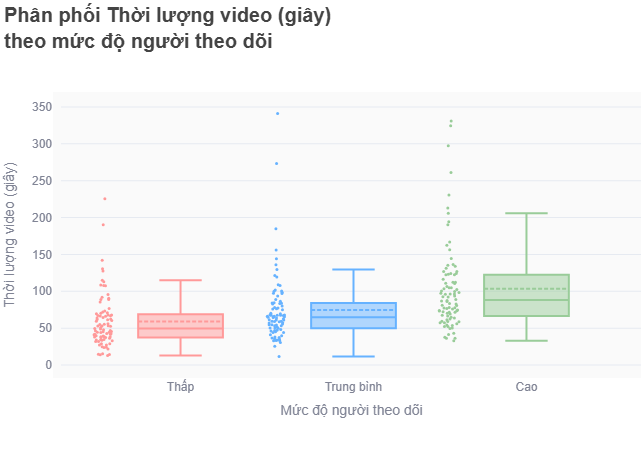
\includegraphics[width=0.7\textwidth]{img/thoi_luong_video_theo_muc_do_nguoi_theo_doi.png}}
    \caption{Phân phối Thời Lượng Video theo Mức Độ Người Theo Dõi}
    \label{fig:thoi_luong_phan_phoi}
\end{figure}

\begin{figure}[H]
    \centering
    \fcolorbox{gray}{white}{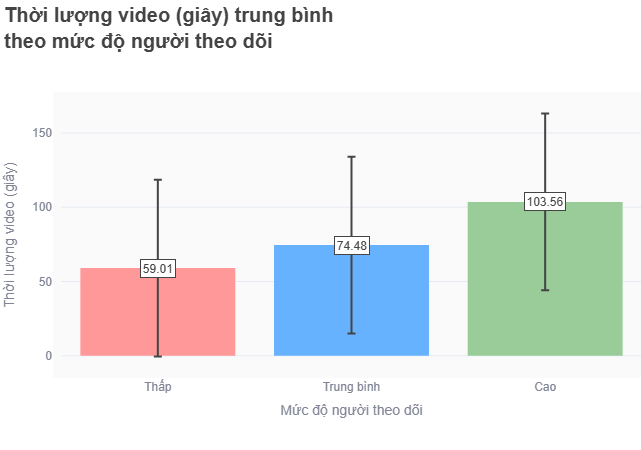
\includegraphics[width=0.7\textwidth]{img/thoi_luong_video_trung_binh_theo_muc_do_nguoi_theo_doi.png}}
    \caption{Thời Lượng Video Trung Bình theo Mức Độ Người Theo Dõi}
    \label{fig:thoi_luong_trung_binh}
\end{figure}

\begin{table}[H]
    \centering
    \begin{tabular}{lccccc}
        \toprule
        Mức độ người theo dõi & Số lượng mẫu & Trung bình & Độ lệch chuẩn & Tối thiểu & Tối đa \\
        \midrule
        Thấp & 87 & 59.01 & 36.30 & 6.00 & 239.00 \\
        Trung bình & 87 & 74.48 & 47.10 & 7.00 & 298.00 \\
        Cao & 90 & 103.56 & 59.60 & 10.00 & 599.00 \\
        \bottomrule
    \end{tabular}
    \caption{Thống kê Mô tả Thời Lượng Video (giây) theo Mức Độ Người Theo Dõi}
    \label{tab:thoi_luong_thong_ke}
\end{table}

\paragraph{Kết quả kiểm định thống kê:}
Kiểm định Kruskal-Wallis: $p$-value = 0.0000
\begin{itemize}
    \item \textbf{Kết luận:} Có sự khác biệt có ý nghĩa thống kê về Thời lượng video (giây) giữa các nhóm người dùng có số lượng người theo dõi khác nhau ($p = 0.0000 < 0.05$).
\end{itemize}

\paragraph{Nhận xét:}
\begin{itemize}
    \item \textbf{Sự khác biệt có ý nghĩa thống kê:} Kết quả kiểm định Kruskal-Wallis với $p$-value = 0.0000 cho thấy có sự khác biệt có ý nghĩa thống kê về thời lượng video giữa các nhóm người theo dõi (Thấp, Trung bình, Cao).
    
    \item \textbf{Thời lượng video và số lượng người theo dõi:} Nhóm người theo dõi \textbf{Cao} có thời lượng video trung bình cao nhất (103.56 giây), tiếp theo là nhóm \textbf{Trung bình} (74.48 giây), và cuối cùng là nhóm \textbf{Thấp} (59.01 giây). Điều này cho thấy, xu hướng chung là người dùng có nhiều người theo dõi hơn có xu hướng đăng tải video dài hơn.
    
    \item \textbf{Ý nghĩa đối với nhà sáng tạo nội dung:} Kết quả này gợi ý rằng việc tăng thời lượng video có thể liên quan đến việc thu hút và giữ chân người xem, đặc biệt là đối với những tài khoản đã có lượng người theo dõi đáng kể. Tuy nhiên, cần lưu ý rằng mối quan hệ này có thể không phải là nguyên nhân - hệ quả. Có thể những người đã thành công với nội dung dài, dẫn đến thu hút nhiều người theo dõi hơn.
\end{itemize}

\paragraph{Chiến lược:}
\begin{itemize}
    \item \textbf{Đối với nhà sáng tạo mới:} Nên thử nghiệm với nhiều độ dài video khác nhau để xem loại video nào thu hút và giữ chân khán giả.
    
    \item \textbf{Đối với nhà sáng tạo có lượng người theo dõi nhất định:} Có thể cân nhắc tăng thời lượng video, nhưng cần đảm bảo nội dung đủ hấp dẫn và giá trị để giữ chân người xem. Cần theo dõi kỹ các chỉ số tương tác như lượt xem, thời gian xem trung bình để đánh giá hiệu quả của việc thay đổi thời lượng video.
\end{itemize}


% --- NỘI DUNG TÀI LIỆU KỸ THUẬT  ---

\subsection{Tổng quan Kỹ thuật}

Phần này cung cấp cái nhìn tổng quan kỹ thuật toàn diện về một bộ các bảng (dashboards) dựa trên \texttt{Streamlit}, được thiết kế để phân tích đa dạng các khía cạnh của dữ liệu người dùng và video trên TikTok. Các ứng dụng này cho phép:

\begin{itemize}
    \item \textbf{Phân tích Tương quan và Phân phối Chỉ số Người dùng:} Khám phá mối quan hệ và sự phân bổ của các chỉ số người dùng cốt lõi như số lượng người theo dõi, tổng lượt thích (tim) và số lượng video đã đăng.
    \item \textbf{Phân tích Tương tác theo Cấp độ Người theo dõi:} Đánh giá mối quan hệ giữa số lượng video và các chỉ số tương tác trên mỗi video (lượt xem, lượt thích, bình luận, chia sẻ) và so sánh các mẫu sáng tạo nội dung (tần suất video, sử dụng hashtag, thời lượng video) giữa các nhóm người dùng có số lượng người theo dõi thấp, trung bình và cao.
    \item \textbf{Phân tích Chi tiết TikToker Cá nhân:} Đi sâu vào dữ liệu video của một TikToker cụ thể, bao gồm lịch sử đăng bài, số liệu tương tác, sở thích cá nhân (hashtag, âm nhạc), và đặc trưng nội dung (chủ đề, giọng điệu, cấu trúc).
    \item \textbf{Phân tích Người dùng TikTok Hàng đầu:} Xác định và trực quan hóa những người dùng TikTok hàng đầu dựa trên các chỉ số như lượt thích, số lượng video, số người theo dõi và tỷ lệ tương tác.
\end{itemize}

Các bảng điều khiển này tận dụng khả năng trực quan hóa dữ liệu tương tác của \texttt{Plotly}, xử lý và phân tích dữ liệu hiệu quả với \texttt{Pandas}, cung cấp thông tin chi tiết dựa trên AI thông qua \texttt{Google Gemini API}, và trong một số trường hợp, sử dụng \texttt{SciPy} cho các kiểm định thống kê. Giao diện người dùng được tùy chỉnh để nâng cao trải nghiệm và cung cấp các tính năng tương tác để khám phá dữ liệu.



\subsubsection{Nguồn Dữ liệu}

\paragraph{Định dạng Tệp:}
Dữ liệu đầu vào chủ yếu được đọc từ các tệp Parquet để tối ưu hiệu suất, với tùy chọn đọc từ tệp CSV.

\paragraph{Đường dẫn Tệp Ví dụ:}
\begin{itemize}
    \item \texttt{data/processed/cleaned\_user\_info.parquet}: Chứa thông tin tổng hợp của người dùng (sử dụng cho phân tích tương quan, phân tích tương tác, và phân tích người dùng hàng đầu).
    
    \item \texttt{data/processed/cleaned\_video\_info.parquet}: Chứa thông tin chi tiết của từng video (sử dụng cho phân tích TikToker cá nhân).
    
    \item \texttt{data/processed/content\_features\_6\_users.parquet}: Chứa các đặc trưng về nội dung được phân tích trước (ví dụ: chủ đề, giọng điệu) cho một số người dùng (sử dụng cho phân tích TikToker cá nhân).
\end{itemize}


\paragraph{Cấu trúc Dữ liệu Chính:}

% Bổ sung mô tả tiếng Việt cho các biến
\begin{longtable}{|w{c}{2.8cm}|p{4.8cm}|p{8cm}|}
\caption{Danh sách các biến phân tích và ý nghĩa}
\label{tab:variables_description} \\
\hline
\textbf{Nhóm Biến} & \textbf{Tên Biến} & \textbf{Ý nghĩa} \\
\hline
\endfirsthead

\hline
\textbf{Nhóm Biến} & \textbf{Tên Biến} & \textbf{Ý nghĩa} \\
\hline
\endhead

\hline
\multicolumn{3}{r}{\textit{(tiếp theo trang sau)}} \\
\endfoot

\hline
\endlastfoot

\multirow{4}{*}{\makecell{Thông tin\\Người dùng}} 
    & \texttt{user.uniqueId} & ID duy nhất của người dùng TikTok \\
    & \texttt{stats.followerCount} & Số lượng người theo dõi \\
    & \texttt{stats.heartCount} & Tổng số lượt thích (thả tim) của người dùng \\
    & \texttt{stats.videoCount} & Tổng số video đã đăng \\
\hline
\pagebreak

\multirow{5}{*}{\makecell{Chỉ số\\Tương tác\\Trung bình}} 
    & \texttt{avg\_comments\_per\_video} & Số bình luận trung bình mỗi video \\
    & \texttt{avg\_diggs\_per\_video} & Số lượt thích trung bình mỗi video \\
    & \texttt{avg\_plays\_per\_video} & Số lượt xem trung bình mỗi video \\
    & \texttt{avg\_shares\_per\_video} & Số lượt chia sẻ trung bình mỗi video \\
    & \texttt{avg\_collects\_per\_video} & Số lượt lưu trung bình mỗi video \\
\hline
\multirow{3}{*}{\makecell{Chỉ số\\Nội dung}} 
    & \texttt{avg\_videos\_per\_week} & Số video trung bình mỗi tuần \\
    & \texttt{avg\_hashtags\_per\_video} & Số hashtag trung bình mỗi video \\
    & \texttt{avg\_video\_duration} & Thời lượng trung bình mỗi video (giây) \\
\hline
\multirow{4}{*}{\makecell{Thông tin\\Video\\Chi tiết}} 
    & \texttt{createTime} & Thời điểm video được đăng \\
    & \texttt{hashtags} & Danh sách các hashtag được sử dụng \\
    & \texttt{music.authorName} & Tên tác giả của âm nhạc trong video \\
    & \texttt{desc} & Mô tả nội dung video \\
\hline
\multirow{5}{*}{\makecell{Đặc trưng\\Nội dung/\\Kịch bản}} 
    & \texttt{main\_content\_focus} & Chủ đề chính của video \\
    & \texttt{structure\_style} & Kiểu cấu trúc nội dung (kể chuyện, mô tả,...) \\
    & \texttt{hook\_type} & Kiểu câu mở đầu thu hút người xem \\
    & \texttt{tone\_of\_voice} & Tông giọng sử dụng trong video \\
    & \texttt{pacing} & Tốc độ trình bày nội dung \\
\hline
\multirow{2}{*}{\makecell{Chỉ số\\Tính toán}} 
    & \texttt{engagement\_rate} & Tỷ lệ tương tác trên tổng số lượt xem \\
    & \texttt{engagement\_ratio} & Tỷ lệ tương tác trên tổng số người theo dõi \\
\end{longtable}


\subsubsection{Hằng số}

\noindent
Các hằng số được định nghĩa để đảm bảo tính nhất quán và khả năng tái sử dụng:

\begin{itemize}
    \item \texttt{DARK\_GRAY}: Mã màu (ví dụ: \texttt{\#444444}) cho văn bản, tiêu đề và các yếu tố trực quan.
    \item \texttt{CLEANED\_USER\_DATA\_FILE}, \texttt{CLEANED\_VIDEO\_INFO\_FILE}, \texttt{CONTENT\_FEATURES\_FILE}: Đường dẫn đến các tệp dữ liệu.
    \item \texttt{COLORS\_RGBA}: Danh sách các mã màu RGBA cho trực quan hóa (ví dụ: xanh dương, đỏ, xanh lá).
    \item \texttt{METRICS}: Danh sách các tên cột \texttt{DataFrame} để phân tích (ví dụ: \texttt{stats.followerCount}).
    \item \texttt{METRIC\_LABELS}: Nhãn tiếng Việt dễ đọc cho các chỉ số (ví dụ: Số người theo dõi).
    \item \texttt{COLUMN\_TO\_AXIS\_TITLE}: Từ điển ánh xạ tên cột sang nhãn trục biểu đồ.
    \item \texttt{COLUMN\_LABELS}, \texttt{COLUMN\_METRICS}: Ánh xạ các trường dữ liệu và chỉ số sang nhãn tiếng Việt.
    \item \texttt{STAT\_TYPES}: Các loại thống kê (ví dụ: \texttt{count}, \texttt{mean}, \texttt{median}).
    \item \texttt{CHART\_OPTIONS}: Ánh xạ các lựa chọn chỉ số sang tên cột, bảng màu và nhãn trục.
\end{itemize}

% \subsection{Thành phần Chức năng}

\subsubsection{Hàm Tiện ích Chung}

Các hàm này xử lý các hoạt động cốt lõi, được chia sẻ hoặc có cấu trúc tương tự giữa các bảng điều khiển:

\begin{itemize}
    \item \texttt{load\_user\_data()} / \texttt{load\_data()}: Tải dữ liệu từ tệp Parquet (hoặc CSV). Chuyển đổi các cột thời gian nếu cần. Thường được lưu trữ đệm với \texttt{@st.cache\_data} (có thể kèm \texttt{persist="disk"}).
    
    \item \texttt{generate\_insights(prompt, api\_key)}: Truy vấn Gemini API để tạo văn bản phân tích dựa trên một \texttt{prompt}. Xử lý ngoại lệ và trả về chuỗi rỗng nếu thất bại. Được lưu trữ đệm với \texttt{@st.cache\_data}.
    
    \item \texttt{display\_AI\_generated\_insights(prompt, api\_key, ...)}: Hiển thị các phân tích do AI tạo ra trong một \texttt{st.expander} của Streamlit, thường có một \texttt{st.spinner} để phản hồi người dùng trong quá trình tải.
    
    \item \texttt{apply\_styles(), } \texttt{personal\_styles()}: Chèn CSS tùy chỉnh để cải thiện giao diện của bảng điều khiển (ví dụ: kiểu chữ tiêu đề, màu nút, định dạng \texttt{expander}) sử dụng \texttt{st.mark-\\down(unsafe\_allow\_html=True)}.
    
    \item \texttt{calculate\_engagement\_ratio(df)}: Tính toán tỷ lệ tương tác, ví dụ: \texttt{stats.heartCount / stats.followerCount} hoặc \texttt{stats.heartCount / stats.videoCount}. Xử lý các trường hợp chia cho không. Được lưu trữ đệm.
\end{itemize}

\subsubsection{Hàm Tiện ích và Trực quan hóa theo Chức năng Bảng Điều khiển}

\noindent
Mỗi bảng điều khiển có các hàm chuyên biệt cho mục đích phân tích của nó:

\paragraph{Phân tích Tương quan và Phân phối Chỉ số Người dùng}
\begin{itemize}
    \item \texttt{get\_correlation\_matrix(df)}: Tính ma trận tương quan Pearson.

    \item \texttt{select\_columns(df, columns)}: Chọn các cột cụ thể từ DataFrame.
    
    \item \texttt{create\_scatter\_matrix(df, template)}: Tạo ma trận biểu đồ phân tán với biểu đồ tần suất trên đường chéo. Tùy chỉnh màu sắc, thêm đường hồi quy.
    
    \item \texttt{create\_correlation\_heatmap(df, template)}: Tạo heatmap của ma trận tương quan, thường ẩn tam giác trên. Xuất ma trận tương quan dưới dạng LaTeX cho AI prompt.
    
    \item \texttt{create\_histogram(df, metric, bins, log\_scale, ...)}: Tạo biểu đồ tần suất với biểu đồ hộp biên. Hỗ trợ tùy chỉnh số lượng \texttt{bins} và thang logarit.
\end{itemize}


\paragraph{Phân tích Tương tác theo Cấp độ Người theo dõi}
\begin{itemize}
    \item \codettt{calculate\_avg\_likes\_per\_video(df)}: Tính trung bình lượt thích trên mỗi video.

    \item \codettt{calculate\_percentiles(df,percentiles)}: Tính các điểm phân vị cho \codettt{stats.follower-\\Count} để xác định ngưỡng thấp, trung bình, cao.
    
    \item \codettt{filter\_data(df, follower\_level, ...)}: Lọc DataFrame dựa trên cấp độ người theo dõi.
    
    \item \codettt{categorize\_by\_followers(df)}: Gán nhãn cấp độ người theo dõi (thấp, trung bình, cao).
    
    \item \codettt{plot\_engagement\_scatter(df, x\_col, y\_col, color)}: Tạo biểu đồ phân tán với đường xu hướng OLS (thường trên thang logarit) và hiển thị hệ số tương quan Pearson.
    
    \item \textit{Biểu đồ hộp và biểu đồ cột:} Được dùng để so sánh các chỉ số (ví dụ: \codettt{avg\_videos\_per\_week}) giữa các nhóm người theo dõi. Biểu đồ cột thường có thanh lỗi (error bars).
    
    \item \textit{Kiểm định Kruskal-Wallis:} Được sử dụng để so sánh sự khác biệt thống kê giữa các nhóm người theo dõi.
\end{itemize}

\paragraph{Phân tích Chi tiết TikToker Cá nhân}
\begin{itemize}
    \item \codettt{filter\_data\_by\_user\_id(cleaned\_video\_info\_df, ..., user\_id)}: Lọc dữ liệu theo \codettt{userId} đã chọn.
    
    \item \codettt{plot\_overall\_posting\_history(video\_counts)}: Tạo biểu đồ diện tích thể hiện lịch sử đăng bài theo ngày, đánh dấu ngày có số lượng video cao nhất.
    
    \item \codettt{calculate\_metrics(video\_df)}: Tính toán các chỉ số hiệu suất chi tiết cho TikToker (ví dụ: tỷ lệ tương tác, lượt xem/lượt theo dõi).
    
    \item \codettt{determine\_level(value, ref\_range)}: Phân loại giá trị thành Thấp, Trung bình, Cao dựa trên khoảng tham chiếu.
    
    \item \codettt{display\_dynamic\_metrics\_dashboard(video\_df)}: Hiển thị bảng điều khiển với các đồng hồ đo (ví dụ: \codettt{go.Indicator}) cho các chỉ số hiệu suất, với màu sắc thay đổi theo mức độ.
    
    \item \codettt{plot\_bar\_chart(df, field, metric, stat\_type, ...)}: Tạo biểu đồ cột ngang hiển thị thống kê theo trường và chỉ số, thường được sắp xếp.
    
    \item \codettt{analyze\_scripts(data\_df, title, user\_context)}: Chức năng chính để phân tích và trực quan hóa đặc trưng nội dung, bao gồm bộ lọc đa lựa chọn, bảng điều khiển số liệu, biểu đồ cột, biểu đồ bánh (hashtags), và biểu đồ phân phối thời lượng.
    
    \item \textit{Heatmap Lịch:} Hiển thị tần suất đăng bài theo ngày trong tuần và giờ trong ngày hoặc ngày trong tháng.
    
    \item \textit{Treemap:} Hiển thị các hashtag phổ biến nhất.
\end{itemize}

\paragraph{Phân tích Người dùng TikTok Hàng đầu}
\begin{itemize}
    \item \codettt{filter\_top\_n\_users(df, metric, n, sort\_order)}: Lọc top N người dùng theo chỉ số được chọn và thứ tự sắp xếp.

    \item \codettt{create\_bar\_chart(data, metric, color\_scale, y\_label)}: Tạo biểu đồ cột hiển thị giá trị chỉ số cho top N người dùng, với thang màu động.
    
    \item \codettt{create\_pie\_chart(data, metric)}: Tạo biểu đồ tròn hiển thị phân phối chỉ số trong top N người dùng.
\end{itemize}

\subsubsection{Bố cục Chung của các Bảng Điều khiển}

\noindent
Mặc dù mỗi bảng điều khiển có bố cục riêng, nhưng chúng cũng có một số cấu trúc chung:

\begin{itemize}
    \item \textbf{Tiêu đề và Mô tả:} Sử dụng \codettt{st.title}, \codettt{st.header}, \codettt{st.markdown} hoặc \codettt{st.write} để giới thiệu mục đích của bảng điều khiển.

    \item \textbf{Thanh bên (Sidebar) / Khu vực Bộ lọc:}
    \begin{itemize}
        \item Cho phép người dùng lựa chọn (chẳng hạn như: \codettt{st.selectbox} để chọn TikToker, chỉ số; \codettt{st.slider} để chọn số lượng người dùng N hoặc phạm vi ngày).
        \item Các nút điều khiển như nút radio (\codettt{st.radio}) để chọn thứ tự sắp xếp.
    \end{itemize}
    
    \item \textbf{Khu vực Hiển thị Chính:}
    \begin{itemize}
        \item \textbf{Tổng quan Dữ liệu/Số liệu Thống kê:} Thường sử dụng \codettt{st.metric} trong các cột (\codettt{st.columns}) để hiển thị các số liệu chính.
    
        \item \textbf{Trực quan hóa Dữ liệu:} Các biểu đồ Plotly được hiển thị bằng \codettt{st.plotly\_chart}. Bố cục có thể là một cột hoặc nhiều cột.
        
        \item \textbf{Phân tích AI:} Các nhận xét từ Gemini API thường được hiển thị trong \codettt{st.expander}.
        
        \item \textbf{Bảng Dữ liệu Chi tiết:} Dữ liệu dạng bảng (thường là DataFrame của Pandas) có thể được hiển thị trực tiếp, trong \codettt{st.expander}, hoặc với phân trang tùy chỉnh.
        
        \item \textbf{Tải Dữ liệu:} Nút \codettt{st.download\_button} để người dùng tải xuống dữ liệu đã xử lý hoặc đã lọc dưới dạng CSV.
    \end{itemize}
\end{itemize}



% \subsection{Chi tiết Triển khai}

\subsubsection{Lưu trữ Đệm (Caching)}

\texttt{@st.cache\_data} được sử dụng rộng rãi để lưu trữ kết quả của các hàm tốn nhiều thời gian xử lý, bao gồm:
\begin{itemize}
    \item Tải dữ liệu (\texttt{load\_user\_data}, \texttt{load\_data}), thường với \texttt{persist="disk"} để lưu trữ giữa các phiên chạy nếu dữ liệu lớn và ít thay đổi.
    
    \item Tính toán ma trận tương quan (\texttt{get\_correlation\_matrix}).
    
    \item Tính toán các chỉ số phức tạp (\texttt{calculate\_engagement\_ratio}, \texttt{calculate\_metrics}).
    
    \item Lọc dữ liệu (\texttt{filter\_data}, \texttt{filter\_top\_n\_users}).
    
    \item Tạo các biểu đồ Plotly (\texttt{create\_scatter\_matrix}, \texttt{create\_bar\_chart}, \dots).
    
    \item Tạo nhận xét AI (\texttt{generate\_insights}).
\end{itemize}
Lưu trữ đệm giúp cải thiện đáng kể hiệu suất và tốc độ phản hồi của ứng dụng khi người dùng tương tác.

\paragraph{\textit{Lưu ý:}} Cần đảm bảo các hàm quan trọng như tải dữ liệu luôn được cache, một số tài liệu gốc chỉ ra đây là điểm có thể cải thiện.


\subsubsection{Tích hợp Trí tuệ Nhân tạo (AI Integration)}

\texttt{Google Gemini API} (thường là mô hình \texttt{gemini-2.0-flash-lite} hoặc tương tự) được sử dụng để tạo ra các nhận xét, phân tích và tóm tắt dựa trên dữ liệu.
    
\paragraph{Cấu trúc Prompts:} Các prompts được thiết kế cẩn thận để cung cấp ngữ cảnh cho AI, có thể bao gồm:
\begin{itemize}
    \item Dữ liệu trực quan hóa (ví dụ: hình ảnh của biểu đồ được chuyển đổi bằng \texttt{fig.to\_image()}).

    \item Bảng dữ liệu tóm tắt (ví dụ: DataFrame được chuyển đổi sang định dạng LaTeX hoặc markdown).
    
    \item Câu hỏi nghiên cứu hoặc hướng dẫn cụ thể về những gì cần phân tích.
    
    \item Các yêu cầu về độ dài hoặc định dạng của phản hồi (ví dụ: tránh các cụm từ như ``\texttt{Dựa trên dữ liệu}'').
\end{itemize}

\paragraph{Xử lý Lỗi:} Các hàm gọi API thường bao gồm khối \texttt{try-except} để xử lý các lỗi tiềm ẩn (ví dụ: API quá tải, lỗi mạng) và cung cấp phản hồi thân thiện cho người dùng.


\subsubsection{Kiểm định Thống kê}

\paragraph{Kiểm định Kruskal-Wallis:} Được sử dụng trong "Bảng Điều khiển Phân tích Tương tác" để so sánh các chỉ số (ví dụ: tần suất đăng bài, sử dụng hashtag, thời lượng video) giữa các nhóm người theo dõi khác nhau (thấp, trung bình, cao). Đây là một kiểm định phi tham số, phù hợp khi giả định về phân phối chuẩn không được đáp ứng.

\paragraph{Xử lý Dữ liệu:} Giá trị \codettt{NaN} thường được loại bỏ trước khi thực hiện kiểm định.

\paragraph{Hiển thị Kết quả:} Giá trị p (p-value) được hiển thị, và kết luận được đưa ra dựa trên mức ý nghĩa (thường là $p < 0.05$).


\subsubsection{Hướng dẫn tương tác trên trang web}

\begin{itemize}
    \item Sử dụng các bộ lọc trong thanh bên hoặc khu vực điều khiển để chọn người dùng, chỉ số, phạm vi ngày, số lượng kết quả (top N), v.v..
    
    \item Xem các biểu đồ tương tác, di chuột qua các điểm dữ liệu để xem chi tiết.
    
    \item Mở rộng các mục "Phân tích AI" hoặc "Chi tiết" để đọc các nhận xét hoặc xem dữ liệu dạng bảng.
    
    \item Sử dụng nút tải xuống để lưu dữ liệu đã lọc.
\end{itemize}

